\chapter{ファイル送信時におけるデータサイズと処理時間の関係について}

まず線形にはならない。高速化するために、いろいろ工夫してある。

\begin{figure}[bpt]\centering
  \begin{center}
    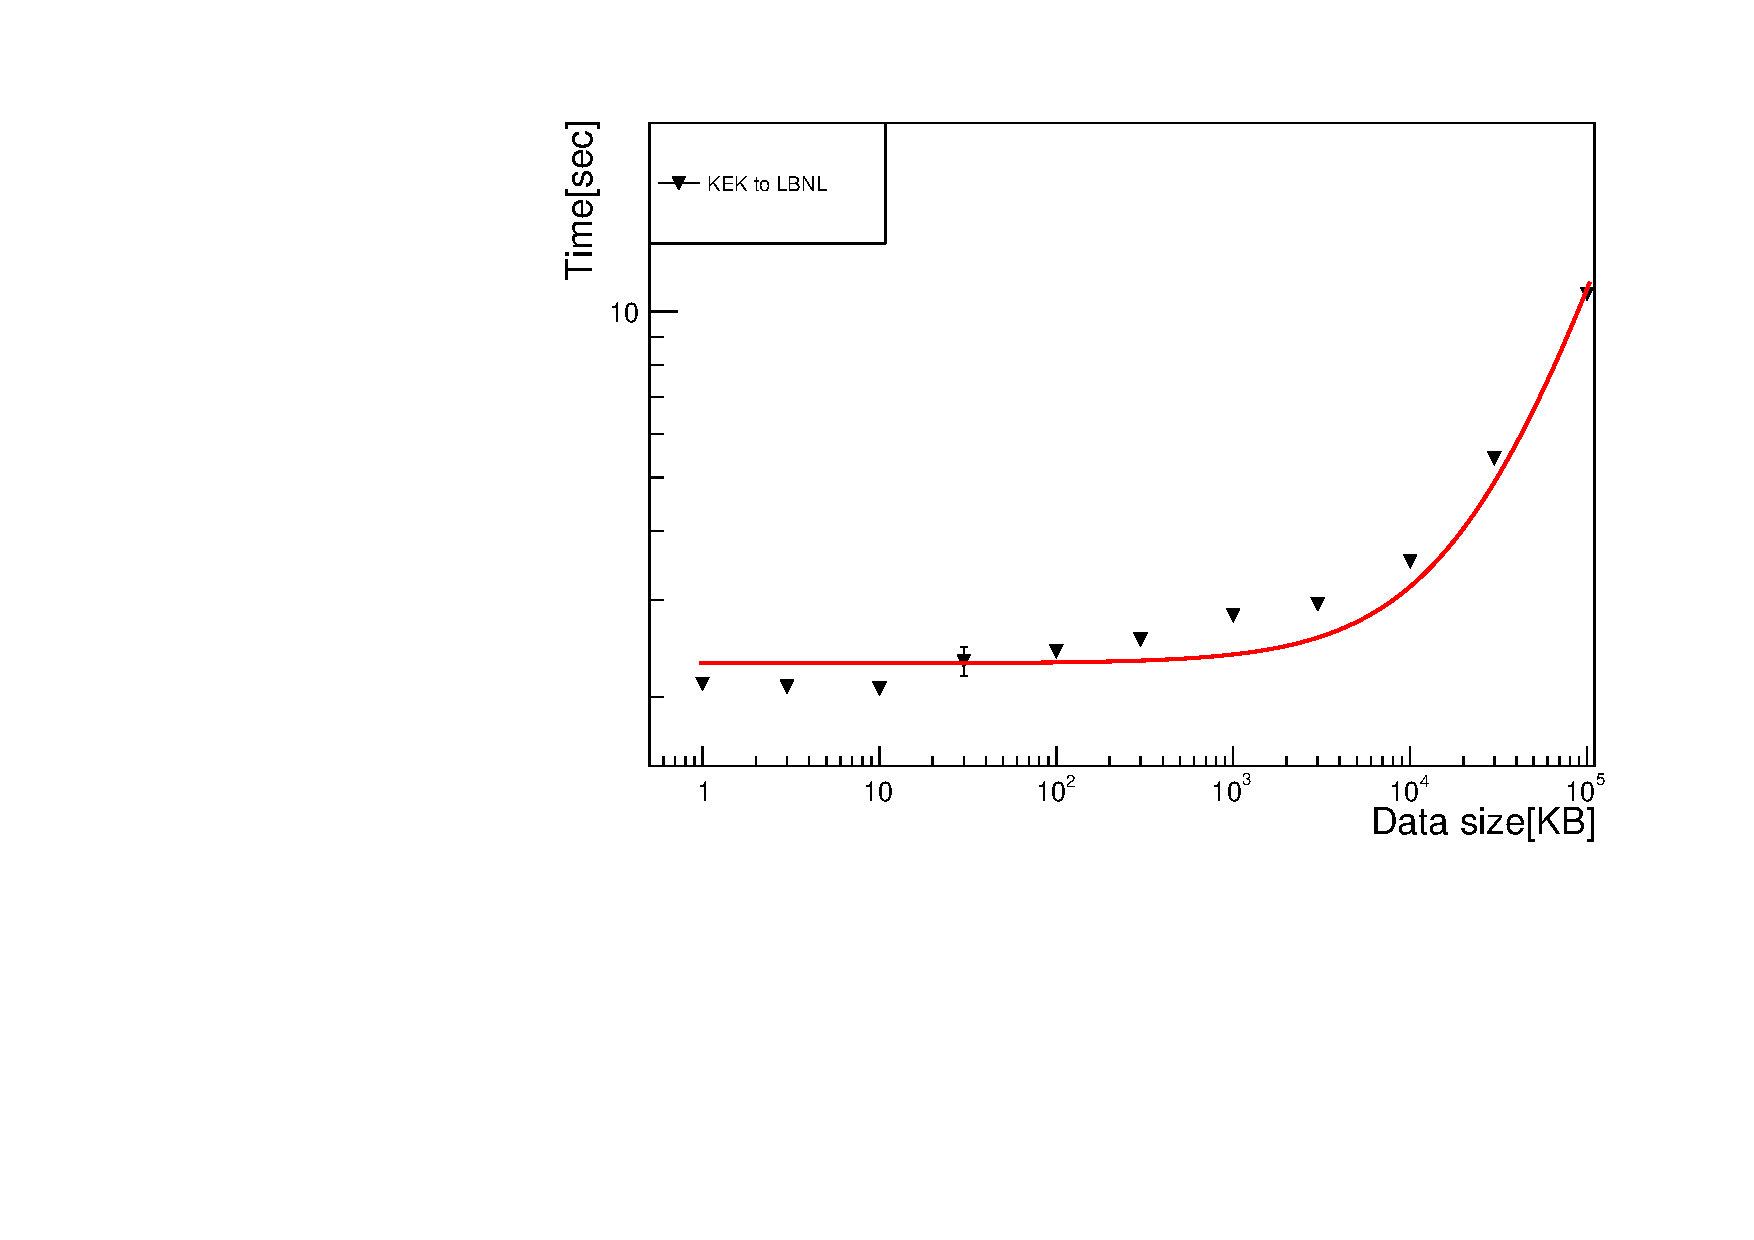
\includegraphics[width=8cm,angle=270]{datasize_vs_time_scp.pdf}
  \caption[添付するファイルサイズと処理時間の関係]{添付するファイルサイズと処理時間の関係}
  \label{datasize_vs_time_scp}
  \end{center}
\end{figure}


Serverのspecは同程度。
Cubic、Window sizeとping(111msec)は変わらない。
一般的には上りより下りの方が太い。
よって、KEKの上りnetworkはLBL上りと比べての方が細いことがわかる。
\begin{figure}[bpt]\centering
  \begin{center}
    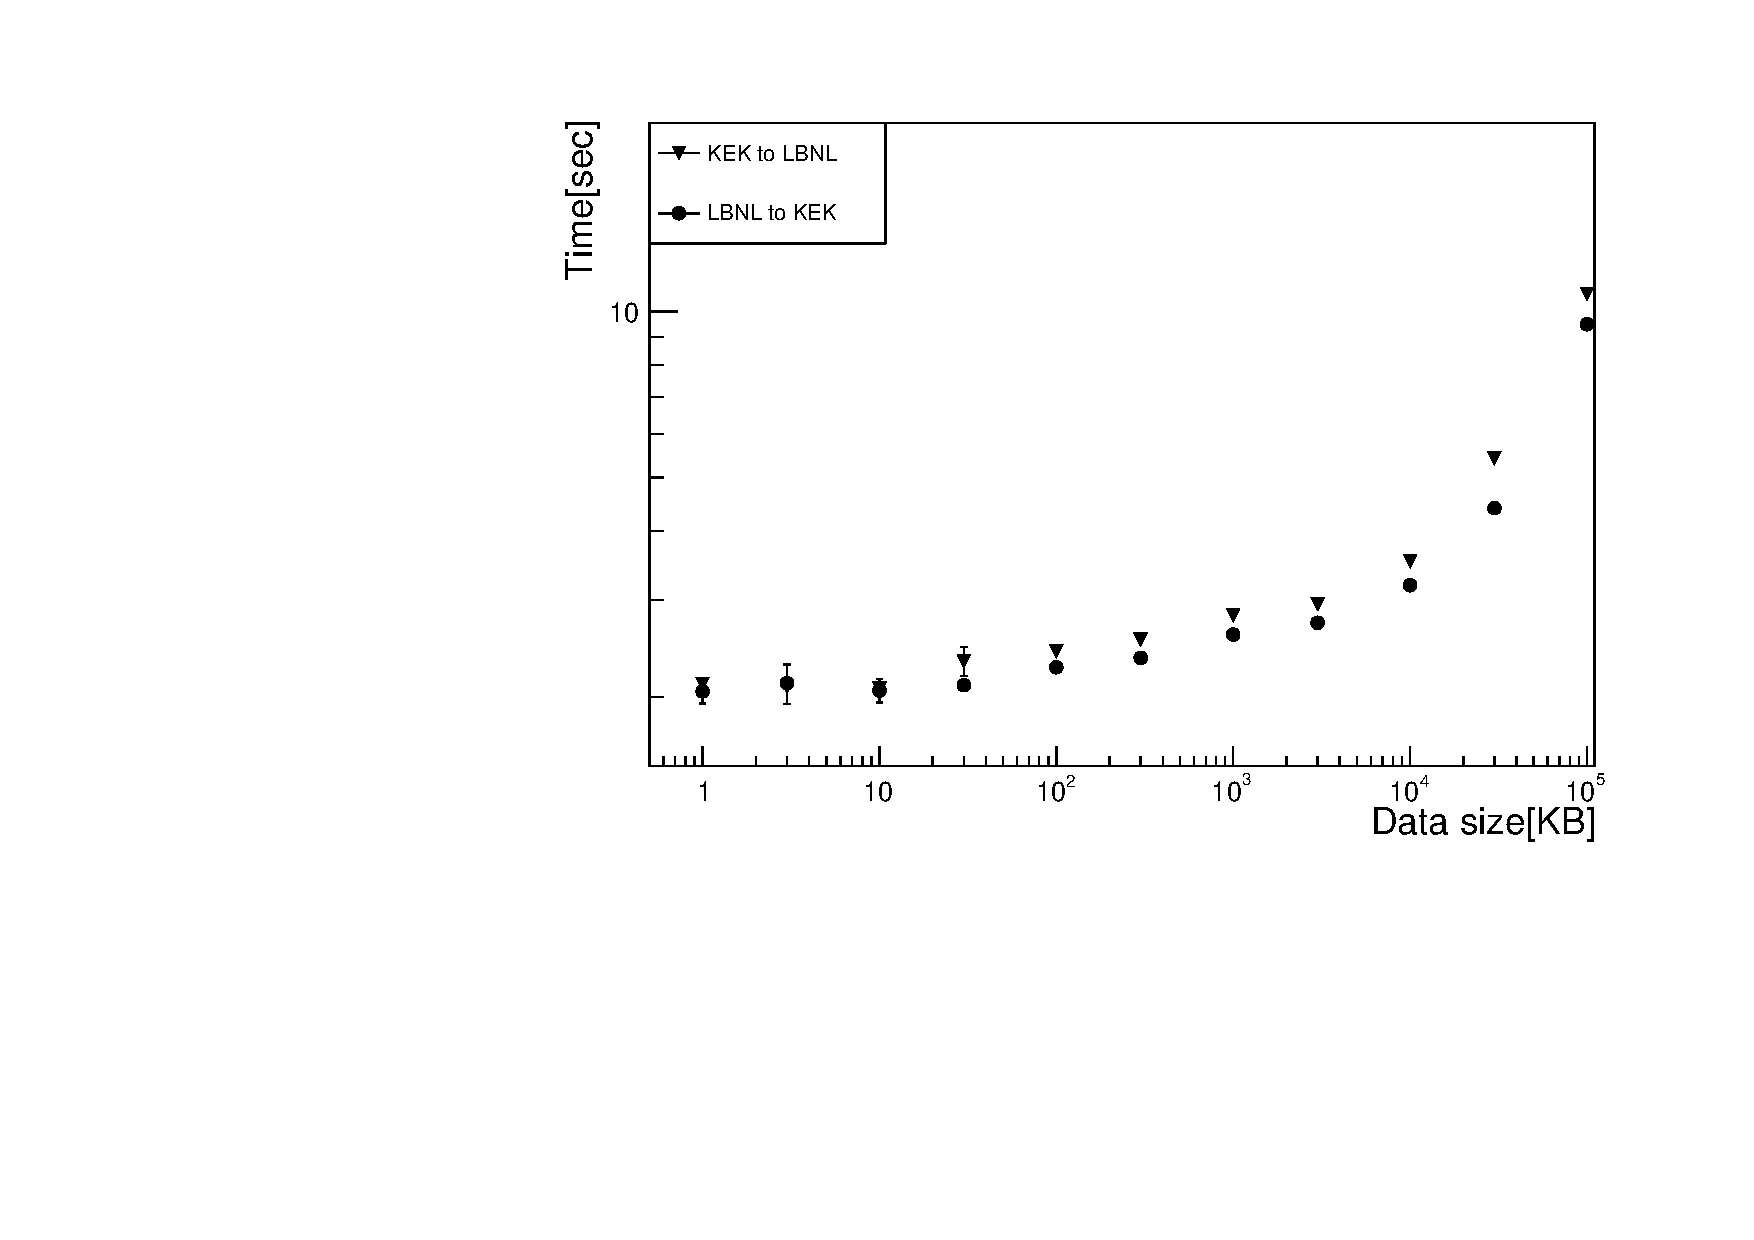
\includegraphics[width=8cm,angle=270]{scp_kek_lbl.pdf}
  \caption[KEK、LBL間のファイル送信]{KEK、LBL間のファイル送信}
  \label{datasize_vs_time}
  \end{center}
\end{figure}

KEKの上りがLBLに比べて細い。
それに加えてRTTがKEKの方が大きいため遅延が広がる。
\begin{figure}[bpt]\centering
  \begin{center}
    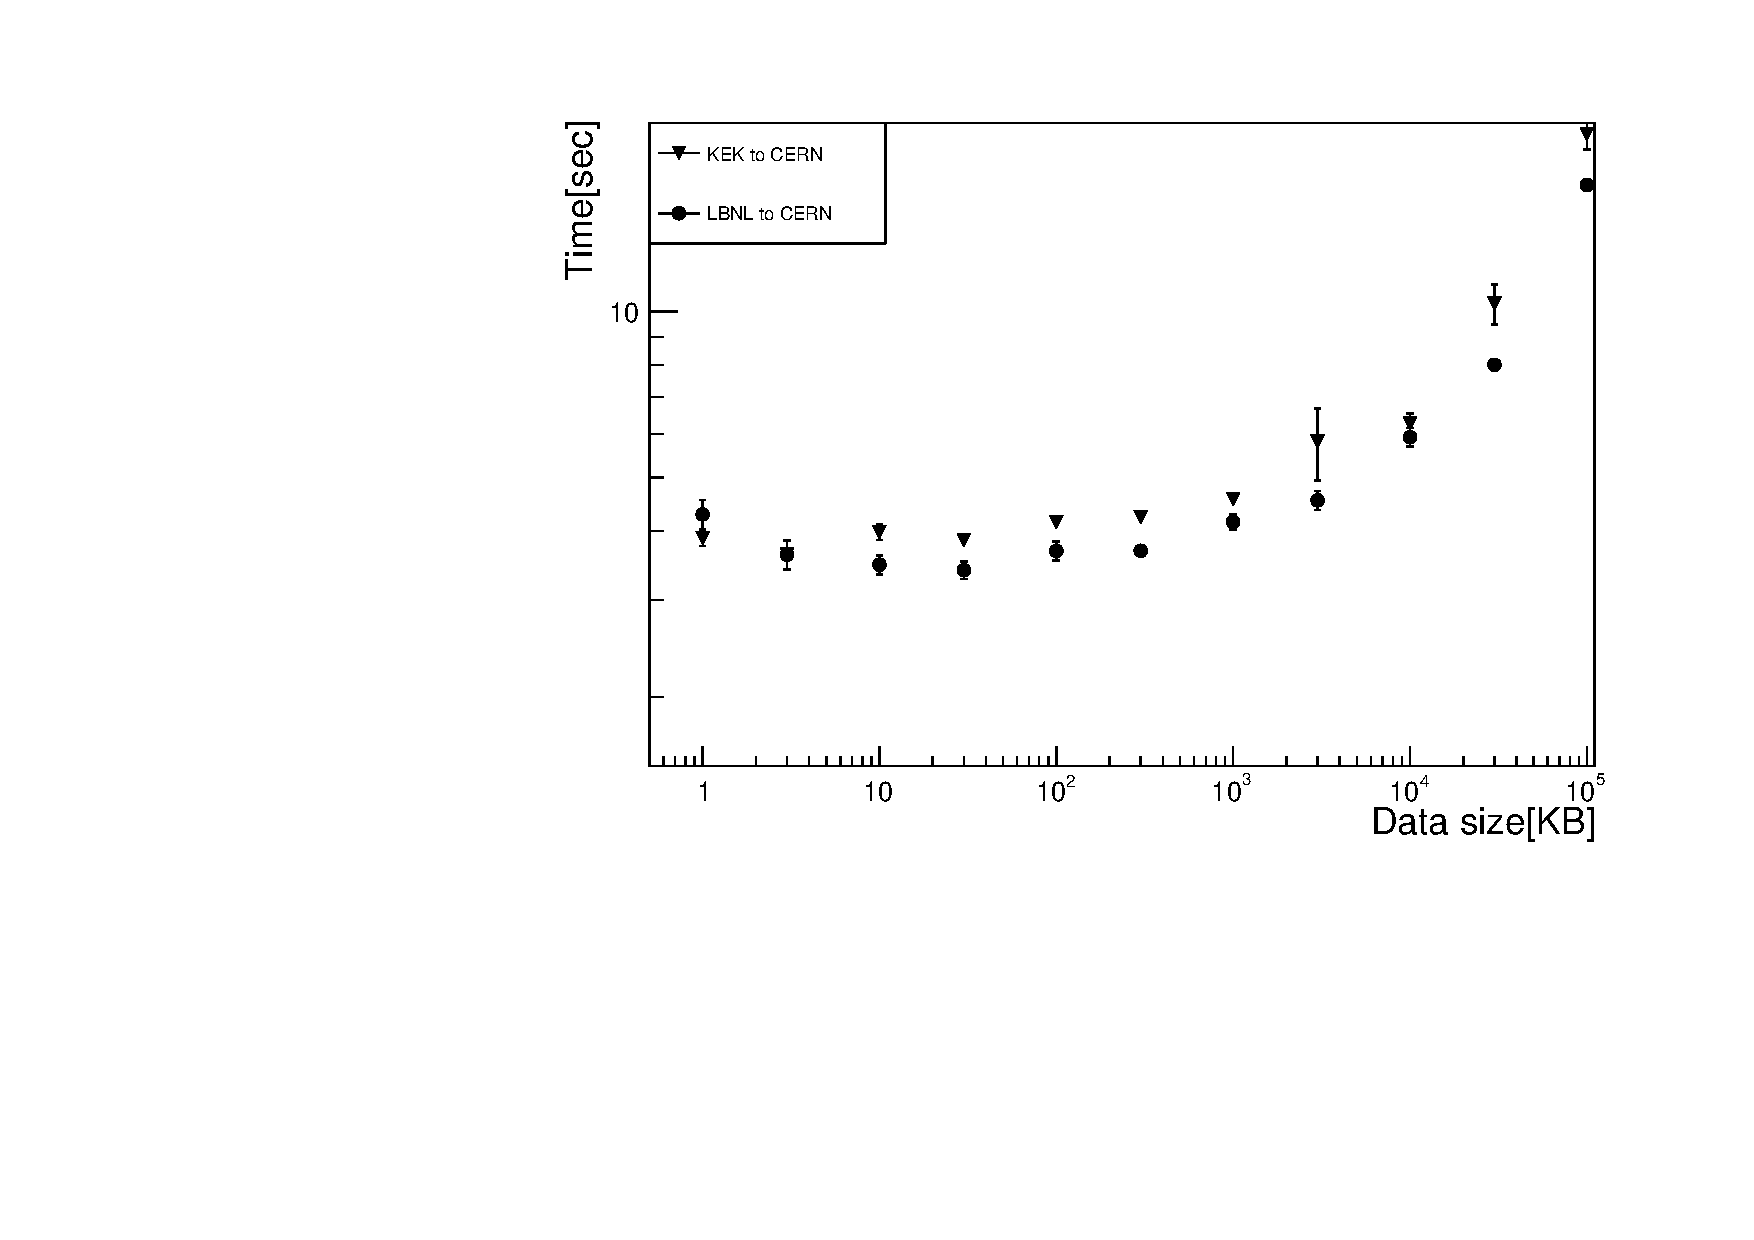
\includegraphics[width=8cm,angle=270]{scp_to_cern.pdf}
  \caption[KEK、LBLとCERN間のファイル送信]{KEK、LBLとCERN間のファイル送信}
  \label{datasize_vs_time}
  \end{center}
\end{figure}


